\section{Analysis of System Survey}
\label{sec:survey:analysis}


In the previous section (\cref{sec:survey:results}), we conducted a data synthesis process on the data we obtained during the systems survey. This process resulted in domain-specific characteristics of identified service mesh systems. In this section, we continue with the data and analyse and discuss notable differences we discovered during the data synthesis process.

The remainder of this section is structured as follows. In \cref{sec:survey:analysis:sm-framework}, we provide a qualitative comparison of the service mesh systems and present several key findings from the obtained data. Thereafter, in \cref{sec:survey:analysis:architectures}, we dive into the different architectures and how they can relate to the observed behaviour. Finally, in \cref{sec:survey:analysis:conclusion}, we provide an answer to \ref{rq-1} and conclude the systems survey.


\subsection{Qualitative Comparison of Service Mesh Systems}
\label{sec:survey:analysis:sm-framework}
% Display resulting framework
% Explain per FR, NFR how it is measured
% Introduction to how it might relate to architecture
% Observations
% - Architecture -> Most Per-Service
% - Traefik Mesh -> No MTLS
% - Three systems fully hit all functional requirements
% - Linkerd2 -> Different Focus

In \cref{tab:result-comparison}, we present a qualitative evaluation of state-of-the-art service mesh systems. In this comparison, we present the architectural style the service proxy uses and map the identified requirements and their level of satisfaction (\cref{sec:survey:results:sm-requirements} to each individual system. 

\begin{table}[!t]

\centering
\resizebox{\linewidth}{!}{ %< auto-adjusts font size to fill line
\begin{tabular}{c|cc|cccc|ccccc}
\toprule

% HEADER 1
\multicolumn{1}{c|}{} &
\multicolumn{2}{c|}{\textbf{Data Plane}} &
\multicolumn{4}{c|}{\textbf{Functional Requirements}} &
\multicolumn{5}{c}{\textbf{Non-Functional Requirements}}  \\

% HEADER 2
\multicolumn{1}{c|}{\textbf{Service Mesh}} &
\multicolumn{1}{c}{\textbf{Service Proxy}}  &
\multicolumn{1}{c|}{\textbf{Proxy Arch.}}  &
\multicolumn{1}{c}{\ref{fr-1}}  &
\multicolumn{1}{c}{\ref{fr-2}}  &
\multicolumn{1}{c}{\ref{fr-3}}  &
\multicolumn{1}{c|}{\ref{fr-4}} &

\multicolumn{1}{c}{\ref{nfr-1}} &
\multicolumn{1}{c}{\ref{nfr-2}} &
\multicolumn{1}{c}{\ref{nfr-3}} &
\multicolumn{1}{c}{\ref{nfr-4}} &
\multicolumn{1}{c}{\ref{nfr-5}} \\

\midrule
% CONTENT

AWS App Mesh
& Envoy         % Service Proxy
& Per-Service   % Proxy Architecture
& \circleF      % FR1 Observability
& \circleF      % FR2 Security
& \circleH      % FR3 Resilience
& \circleF      % FR4 Additional Deployment Models

& \circleH      % NFR1 Application Level Protocol Aware
& \circleE      % NFR2 Open-Source
& \circleF      % NFR3 Documentation
& \circleE      % NFR4 CNCF Level
& \circleE      % NFR5 Commmunity Recognition
\\

Cilium
& Cilium eBPF   % Service Proxy
& In Kernel     % Proxy Architecture
& \circleF      % FR1 Observability
& \circleF      % FR2 Security
& \circleF      % FR3 Resilience
& \circleF      % FR4 Additional Deployment Models

& \circleF      % NFR1 Application Level Protocol Aware
& \circleF      % NFR2 Open-Source
& \circleH      % NFR3 Documentation
& \circleH      % NFR4 CNCF Level
& \circleH      % NFR5 Commmunity Recognition
\\

Consul
& Envoy         % Service Proxy
& Per-Service   % Proxy Architecture
& \circleF      % FR1 Observability
& \circleF      % FR2 Security
& \circleH      % FR3 Resilience
& \circleF      % FR4 Additional Deployment Models

& \circleH      % NFR1 Application Level Protocol Aware
& \circleF      % NFR2 Open-Source
& \circleF      % NFR3 Documentation
& \circleE      % NFR4 CNCF Level
& \circleH      % NFR5 Commmunity Recognition
\\

Ease Mesh
& EaseGress     % Service Proxy
& Per-Service   % Proxy Architecture
& \circleF      % FR1 Observability
& \circleE      % FR2 Security
& \circleH      % FR3 Resilience
& \circleE      % FR4 Additional Deployment Models

& \circleH      % NFR1 Application Level Protocol Aware
& \circleF      % NFR2 Open-Source
& \circleE      % NFR3 Documentation
& \circleE      % NFR4 CNCF Level
& \circleE      % NFR5 Commmunity Recognition
\\

Istio
& Envoy         % Service Proxy
& Per-Service   % Proxy Architecture
& \circleF      % FR1 Observability
& \circleF      % FR2 Security
& \circleF      % FR3 Resilience
& \circleF      % FR4 Additional Deployment Models

& \circleF      % NFR1 Application Level Protocol Aware
& \circleF      % NFR2 Open-Source
& \circleF      % NFR3 Documentation
& \circleE      % NFR4 CNCF Level
& \circleF      % NFR5 Commmunity Recognition
\\

Kuma
& Envoy         % Service Proxy
& Per-Service   % Proxy Architecture
& \circleF      % FR1 Observability
& \circleF      % FR2 Security
& \circleF      % FR3 Resilience
& \circleF      % FR4 Additional Deployment Models

& \circleF      % NFR1 Application Level Protocol Aware
& \circleF      % NFR2 Open-Source
& \circleF      % NFR3 Documentation
& \circleH      % NFR4 CNCF Level
& \circleE      % NFR5 Commmunity Recognition
\\

Linkerd2
& Linkerd2 Proxy% Service Proxy
& Per-Service   % Proxy Architecture
& \circleF      % FR1 Observability
& \circleF      % FR2 Security
& \circleH      % FR3 Resilience
& \circleF      % FR4 Additional Deployment Models

& \circleH      % NFR1 Application Level Protocol Aware
& \circleF      % NFR2 Open-Source
& \circleF      % NFR3 Documentation
& \circleF      % NFR4 CNCF Level
& \circleF      % NFR5 Commmunity Recognition
\\

Nginx Service Mesh
& NGINX Plus    % Service Proxy
& Per-Service   % Proxy Architecture
& \circleF      % FR1 Observability
& \circleF      % FR2 Security
& \circleH      % FR3 Resilience
& \circleE      % FR4 Additional Deployment Models

& \circleH      % NFR1 Application Level Protocol Aware
& \circleE      % NFR2 Open-Source
& \circleH      % NFR3 Documentation
& \circleE      % NFR4 CNCF Level
& \circleE      % NFR5 Commmunity Recognition
\\

Open Service Mesh
& Envoy         % Service Proxy
& Per-Service   % Proxy Architecture
& \circleF      % FR1 Observability
& \circleF      % FR2 Security
& \circleE      % FR3 Resilience
& \circleE      % FR4 Additional Deployment Models

& \circleH      % NFR1 Application Level Protocol Aware
& \circleF      % NFR2 Open-Source
& \circleH      % NFR3 Documentation
& \circleH      % NFR4 CNCF Level
& \circleE      % NFR5 Commmunity Recognition
\\

Traefik Mesh
& Traefik Proxy % Service Proxy
& Per-Node      % Proxy Architecture
& \circleF      % FR1 Observability
& \circleE      % FR2 Security
& \circleH      % FR3 Resilience
& \circleE      % FR4 Additional Deployment Models

& \circleH      % NFR1 Application Level Protocol Aware
& \circleF      % NFR2 Open-Source
& \circleH      % NFR3 Documentation
& \circleE      % NFR4 CNCF Level
& \circleE      % NFR5 Commmunity Recognition
\\
\bottomrule
\end{tabular}
} %< \resizebox

\caption[Qualitative comparison between state-of-the-art \gls{sm} systems.]{Qualitative comparison between state-of-the-art \gls{sm} systems. \\
There are three different symbols in the table, each of them represents how well a requirement is satisfied. \circleF: Fully Satisfied, \circleE: Not Satisfied, \circleH: Partially Satisfied.}
\label{tab:result-comparison}

\end{table}

We now present a list of the most interesting findings we obtained:

\begin{enumerate}[label=\textbf{F\arabic*}, leftmargin=3\parindent]
    \item \textbf{Most of the identified \gls{sm} systems share a similar data plane architecture.}
    \label{f-1}
    % Most use a per-service proxy
    % Most use envoy
    
    The first finding from the obtained data is that most of the systems use a similar architecture for the data plane of the \gls{sm}. Out of the ten identified \gls{sm} implementations, eight used a per-service proxy architecture. Furthermore, out of those eight using a per-service proxy architecture, half of them used the same service proxy implementation in the form of \textit{Envoy}, an open-source general purpose proxy.
    
    \item \textbf{Per-node data plane architecture prevents support for common security features.}
    \label{f-2}
    % Traefik uses per-node
    % Is the only one that does not support the security requirements
    
    The second finding is that only a single identified system used a service proxy architecture, where the service proxy was implemented on a per-node granularity. \textit{Traefik Mesh} is the identified service mesh that used such an architecture, and most notably it was the only implementation that did not support any of the security capabilities listed (\ref{fr-2}). In particular, it does not support automatic mutual TLS encryption between services, a killer feature to enhance the security in any environment. To further elaborate on this, we dive deeper into the characteristics of data plane architectures in the next section (\cref{sec:survey:analysis:architectures}).

    \item \textbf{Most identified systems do not support all functional requirements.}
    \label{f-3}
    % 3/10 implementations support all requirements
    % Cilium, Istio and Kuma
    % Cilium -> Network focus
    % Istio -> Feature focus + Mature + Complex
    % Kuma -> Feature focus, Extensibility, Support for different environments
    
    The third finding is that out of all ten identified service mesh systems, just three systems fully satisfy all the functional requirements (\ref{fr-1}-\ref{fr-4}), namely, \textit{Cilium}, \textit{Istio} and \textit{Kuma}. This finding can be explained by taking a closer look at the maturity levels and the goals that the individual \gls{sm} implementations have. The three identified services that achieve all functional requirements are mature projects or heavily emphasize their feature set and extensibility. \textit{Istio} is the most mature platform, with large backing and is the most used \gls{sm} implementation out of all identified systems according to the \gls{cncf} survey conducted in 2021 \cite{cncf-survey-2021}. It also supports the most features and therefore hits all the functional requirements. \textit{Kuma} on the other hand, is a much smaller project. However, its focus lies on having a broad feature set with lots of extensibility options as well, thus achieving all functional requirements as well. \textit{Cilium} on the other hand, is a new entry in the \gls{sm} landscape (as can be seen by the release date in the list of non-functional attributes (\cref{tab:result-nfa}). However, this story also does not paint the entirety of the picture as it builds upon the \textit{Cilium} networking solution, a mature networking solution that already facilitates most of the functional requirements listed.
    

    \item \textbf{Maturity does not translate to support of requirements.}
    \label{f-4}
    % Linkerd2 Does not hit all requirements
    % Different project focus
    % - Simple
    % - Fast
    % - Tailored proxy, less features
    
    A fourth finding is that maturity does not necessarily translate to the support of functional and non-functional requirements. This refers to \textit{Linkerd2} in particular, which does not  not fully satisfy the resiliency requirements \ref{fr-3} and also lacking in the additional application level protocol support \ref{nfr-1}. Despite its maturity, large-scale usage in production environments \cite{cncf-survey-2021}, and graduated \gls{cncf} project status, the system seems to be lacking in features. This, however, can be attributed to the goals of the project. Whereas \textit{Istio} has the most features of any system, it is also dubbed as a complex system. \textit{Linkerd2}, however, aims to optimize for simplicity and speed. Instead of using a generic proxy with numerous features and capabilities, such as \textit{Envoy} or \textit{NGINX}, it uses a custom proxy specifically tailored to the service mesh, optimizing for simplicity, security, and performance \cite{linkerd-no-envoy}.
    
    \item \textbf{Lack of additional layer 7 protocol support.}
    \label{f-5}
    % 4/10 systems support 'additional' layer 7 protocols
    % Why it is useful
    % External project (Aeraki) -> Tries to solve this
    
    A fifth finding is that just a few of the identified systems support additional application level protocols (\ref{nfr-1}). Since \gls{sm} systems can greatly benefit from additional application level support from its service proxies, it can be a promising area. It can enable application level aware traffic management, rich metric collection or can lead to advanced authorization policies. \textit{Cilium} and \textit{Kuma} for example, provide support for the Apache Kafka protocol and therefore can target specific messages when dealing with events of the platform.  Although we did identify only a few implementations that provided support for this, we did identify an external project in the \gls{cncf} landscape that tries to enable this. \textit{Aeraki}\footnote{\url{https://www.aeraki.net/}}, attempts to close this gap by creating an extensible platform that enables layer 7 support for many protocols such as \textit{Redis}, \textit{Kafka} and \textit{ZooKeeper}. This project, however, only provides support for \textit{Istio} and therefore currently does not support any other \gls{sm} implementation.
    
    \item \textbf{New technologies enable additional data plane architectures.}
    \label{f-6}
    % Single sm uses kernel based proxy (Cilium)
    % - Does not have linear dependency on proxy/service
    % - Relatively new techonology
    
    A final finding is that only a single project uses a kernel-based proxy. \textit{Cilium} uses a kernel-based proxy approach by utilizing \gls{ebpf} applications to implement the service proxy. Together with \textit{Traefik proxy}, it is the only \gls{sm} that does not use a per-service based data plane architecture. We can attribute this finding to the fact that \gls{ebpf} is a relatively new technology, and that the \textit{Cilium} networking project has been banking on that technology before extending its networking solution to include the properties of a service mesh in late 2021 \cite{cilium-mesh}. Although this is a fairly new approach, it has been adopted by one of the leading \gls{k8s} service providers in the form of \textit{Google Kubernetes Engine} \cite{google-cilium-ebpf}. Furthermore, other \gls{sm} systems also experiment with \gls{ebpf} technology to improve upon existing functionalities and support new features \cite{istio-merbridge, nginx-service-mesh-arch}. 
\end{enumerate}


% The first observation we can make from the obtained data is that most of the systems use a data plane with a per-service proxy. However, some \gls{sm} systems use a different approach, such as \textit{Traefik Mesh}, which uses a per-node proxy and \textit{Cilium}, which uses a kernel-based proxy. This can be attributed to the fact that half of the implementations use \textit{Envoy} as proxy, which is an open-source proxy. 

% The second observation that we can make is that \textit{Traefik Mesh} does not support any of the security capabilities listed (\ref{fr-2}). Notably, it does not support automatic mutual TLS encryption between services, a killer feature to enhance the security in any environment. This result, however, is unsurprising if we relate it to the first observation. Due to its per-node proxy, all service-to-service communications travel first from a service to the proxy in a potentially unencrypted state. This allows for potential attackers to intercept this, and thus to create a zero-trust environment application developers have to implement mutual TLS connections manually.

% The third observation is that there are three systems that fully satisfy all the functional requirements (\ref{fr-1}-\ref{fr-4}), namely, \textit{Cilium}, \textit{Istio} and \textit{Kuma}. The first of those systems has a heavy focus on networking and features, as it originates as a networking solution and transcended into the service mesh space since December 2021 \cite{cilium-ebpf-mesh}. The second of those systems can be considered the most mature \gls{sm} system, which sees the most amount of production use according to the \gls{cncf} 2021 survey \cite{cncf-survey-2021} and has enterprise backing. Kuma, on the other hand, is a project with much smaller backing and usage, however it has a focus on extensibility and features, even allowing the system in non-\gls{k8s} or vm-based environments. 

% A fourth observation is that \textit{Linkerd2} does not hit all the functional requirements as it does not fully satisfy the resiliency requirements \ref{fr-3} and also lacking in the additional application level protocol support \ref{nfr-1}. Despite its maturity, large-scale usage in production environments and graduated \gls{cncf} project status, the system seems to be lacking in features. This, however, can be attributed to the goals of the project. Whereas \textit{Istio} has the most features of any system, it is also dubbed as a complex system. \textit{Linkerd2}, however, aims to optimize for simplicity and speed. Instead of using a generic proxy with numerous features and capabilities, such as \textit{Envoy} or \textit{NGINX}, it uses a custom proxy specifically tailored to the service mesh, optimizing for simplicity, security and speed \cite{linkerd-no-envoy}.

% A fifth observation is that additional application level protocol support \ref{nfr-1} exists, however, not many systems have support for it out of the box. Since \gls{sm} systems can greatly benefit from application aware proxies, it can be a promising area. It can enable application level aware traffic management, rich metric collection or can lead to advanced authorization policies. Some proxies like \textit{Cilium} and \textit{Kuma} provide support for protocols such as \textit{Kafka}, in which they can target specific messages. Another project in the \gls{cncf} landscape under the name of \textit{Aeraki} \footnote{\url{https://www.aeraki.net/}}, attempts to close this gap by creating an extensible platform that enables layer 7 support for many protocols such as \textit{Redis}, \textit{Kafka} and \textit{ZooKeeper}. This project, however, only provides support for \textit{Istio} and therefore currently does not support any other \gls{sm} implementation.

% A final observation is that only a single project uses a kernel-based proxy. \textit{Cilium} uses a kernel-based proxy approach by utilizing \gls{ebpf} technology. Together with \textit{Traefik proxy}, it is the only \gls{sm} that does not use a per-service based data plane architecture. The reason for this is that \gls{ebpf} the technology is relatively new, and \textit{Cilium} has been banking on that technology before extending its networking solution to include the properties of a service mesh \cite{cilium-mesh}. Although this is a fairly new concept, it has been adopted by one of the leading \gls{k8s} service provider in the form of \textit{Google Kubernetes Engine} \cite{google-cilium-ebpf}. Furthermore, it is also used for a bleeding edge \textit{Istio} feature \cite{istio-merbridge} and in certain \textit{NGINX Service Mesh} beta features \cite{nginx-service-mesh-arch}.


\subsection{Analysis of Common Service Mesh Architectures}
\label{sec:survey:analysis:architectures}
% Introduce section
% Per-Service Arch
% Per-Node Arch
% Kernel

In this section, we analyse the identified \gls{sm} architectures in more detail. For every identified architecture, we present a reference topology and discuss the advantages and disadvantages one such implementation has. First, in \cref{sec:survey:analysis:architectures:per-service}, we discuss the most common identified approach, a \gls{sm} using a per-service proxy. Next, in \cref{sec:survey:analysis:architectures:per-node}, we discuss architectures leveraging a per-node proxy. Finally, in \cref{sec:survey:analysis:architectures:ebpf}, we discuss architectures using a kernel-based \gls{ebpf} approach.


\subsubsection{Per-Service Proxy}
\label{sec:survey:analysis:architectures:per-service}
% - Simplest architecture
% - Overhead, many proxies
% - Resource Usage
% - Latency / Hops

During the systems survey, we identified ten different \gls{sm} systems. Out of those ten systems, eight of those shared similar architectural characteristics. For all of these systems, we identified that the mesh network was established by introducing a proxy for every individual software service present. This architectural style is so common within the \gls{k8s} ecosystem, that the pattern is often referred to as the \textit{sidecar pattern}.


In \cref{fig:sm-arch-per-service}, we present a reference architecture of this design pattern for service meshes in a \gls{k8s} cluster. This shows the data path of a packet throughout its lifespan in a system that implements this architecture. To explain the data path of a packet, we first introduce the individual components depicted, as most of them are present in the other architectures as well. 

\begin{figure}[!t]
    \centering
    
    \scalebox{.8}{
    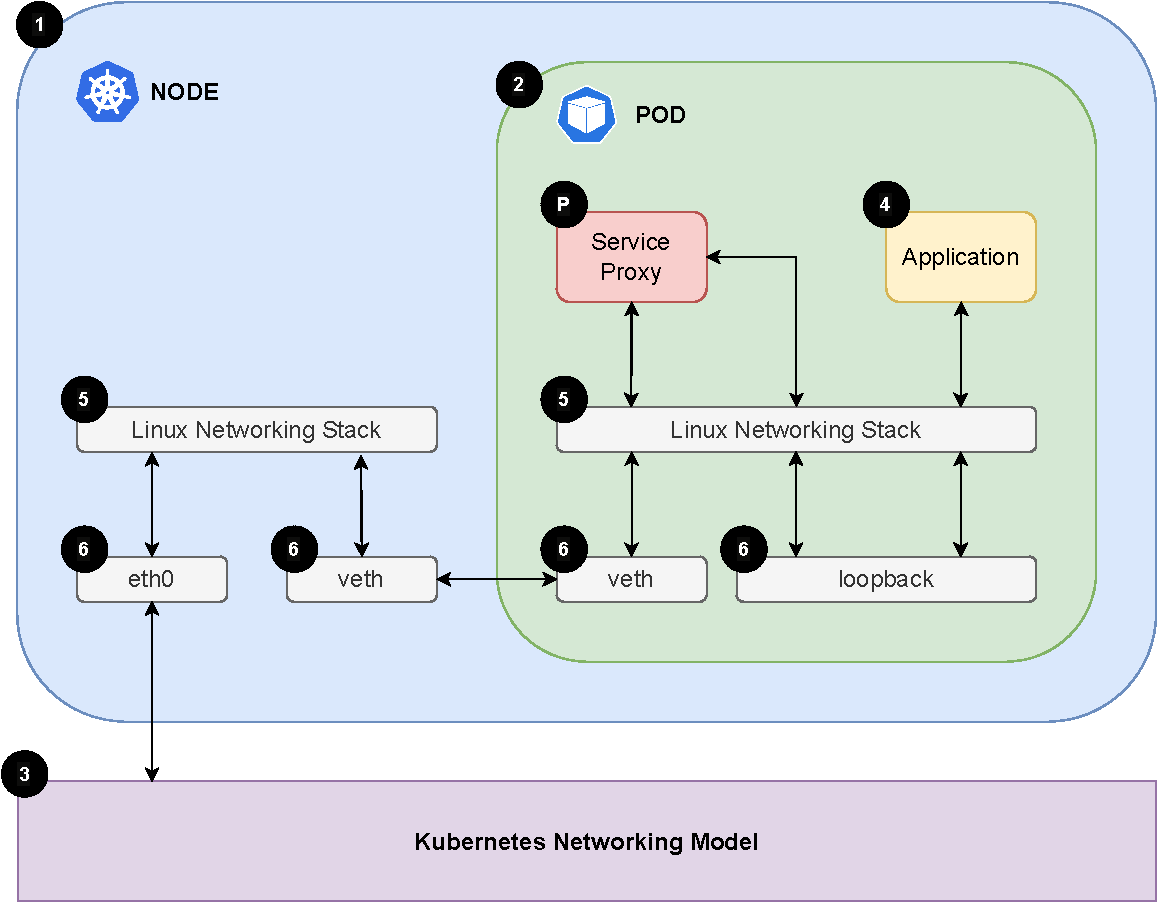
\includegraphics[width=\linewidth]{3_systems_survey/figures/sm-arch-per-service.pdf}
    }

    \caption[Per-service proxy plane architecture.]{The data path of a per-service data plane.}
    \label{fig:sm-arch-per-service}
\end{figure}

% Basic components introduction
First off, we have the node (\designref{1}), this represents a worker machine in \gls{k8s}, which can run workloads. Next up, we have a \gls{pod} (\designref{1}), this is the smallest unit of deployment within \gls{k8s} and consists of one or more application containers. The last \gls{k8s} related concept is the Kubernetes Networking Model (\designref{3}) \cite{kubernetes-cluster-networking}, which can be implemented in various ways, but has as goal to connect the nodes and pods within the cluster. Within the \gls{pod}, lives the actual application (\designref{4}), which can for example be a web server. The \textit{Linux Network Stack} (\designref{5}) is abstracted in this design as one single component, but consists of routing and filtering tables used to manage packets within the system. An important note, is that both the node and the \gls{pod} implement a separate networking stack, which isolates the pod network from the host network through network namespaces \cite{man-network-namespaces}. The traffic flows to physical and virtual network interfaces (\designref{6}) connected through one another, to reach its destination. Note that in actual deployments, more complex models are often present, such as bridge networks to support multiple pod networks or tunnel interfaces to create overlay networks, for instance. However, for this example, the added complexity does not help to illustrate the architectural differences at hand.


% Explain datapath
With the basic components of the reference architecture explained, we can take a closer look at the data path of a service request. Whenever a request to a service has been made that lives within the application pod (\designref{4}) a packet first enters the node. The inbound packet enters through the network interface (\designref{6}), has to pass through the kernel's networking stack (\designref{5}) to reach the \gls{pod}'s network namespace. After this, the traffic will reach the service proxy (\designref{P}) because it is configured to intercept all network traffic inside the pod. From there onwards, it has to travel through a loopback interface to finally reach the application. Replies from the application will traverse a similar, but inverse, data path.

% Advantages/Disadvantages
One of the advantages of such an architecture is that you can have fine-grained control over the traffic, as it is intercepted the moment it enters the namespace of the \gls{pod}. This characteristic allows the security features discussed during this systems review (\ref{fr-2}), and can for example enable encrypted connections between all traffic leaving a \gls{pod}. Furthermore, the \textit{sidecar pattern} allows for a very generic implementation, and does not require much if any modifications from the user's perspective. This enables a user-friendly user experience, while also allowing support for general purpose proxies such as \textit{Envoy} or \textit{HAProxy}. These advantages, make it so that this is the most common architectural approach identified. A disadvantage, however, is that this design introduces additional overhead. First off, it introduces an overhead in system resources, as there now is a network proxy for every software service. Furthermore, it introduces additional latency for the traffic, as for every service request, the packets travel through the proxy twice (ingress/egress).


\subsubsection{Per-Node Proxy}
\label{sec:survey:analysis:architectures:per-node}
% - Less overhead and hops
% - No MTLS

Another identified \gls{sm} architecture makes use of the per-node proxy. This architectural style is used by a single identified \gls{sm} system, \textit{Traefik Mesh}. We present this form of \gls{sm} architecture in \cref{fig:sm-arch-per-node}. Although many of the components in this system are similar and previously explained in \cref{sec:survey:analysis:architectures:per-service}, some differences change several characteristics drastically.

\begin{figure}[!t]
    \centering
    
    \scalebox{.8}{
    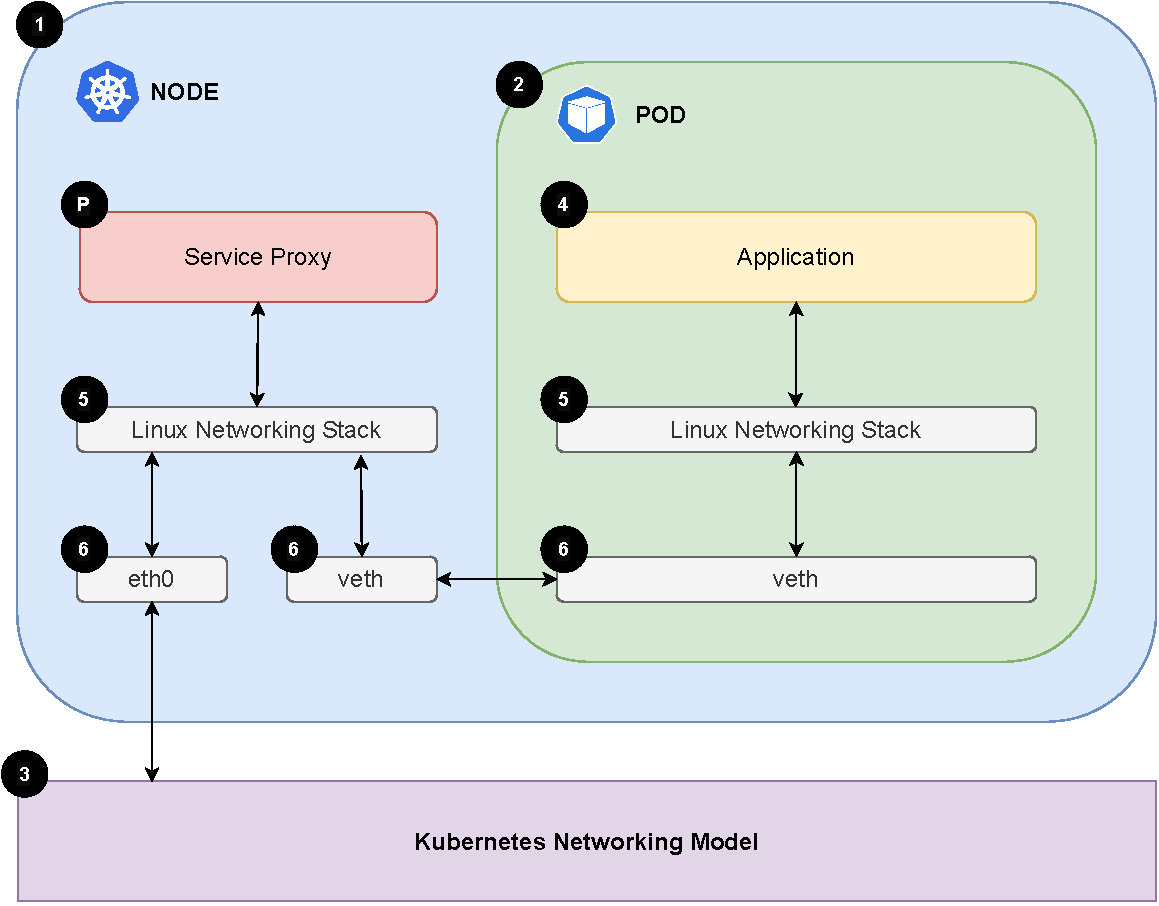
\includegraphics[width=\linewidth]{3_systems_survey/figures/sm-arch-per-node.pdf}
    }
    
    \caption[Per-node proxy plane architecture.]{The data path of a per-node data plane.}
    \label{fig:sm-arch-per-node}
\end{figure}

The most significant difference compared to the per-service architectural style is that service proxy (\designref{P}) is now not embedded within the \gls{pod} but lives within the node, thus makes use of the host network namespace. The reason for this is that this architectural style tries to limit the additional overheads caused by the introduces proxies of a \gls{sm}. This style of service proxies results in a single proxy per node, and thus does not scale linearly with the number of services on a node. This leads to the advantage that it consumes less system resources in the form of CPU cycles and memory. An additional benefit of this approach is that the traffic in the data path now has to traverse the proxy once in a service-to-service request. This halves the amount of service proxy hops compared to the previous solution. 

However, this architectural pattern comes at a cost. Since the traffic is not passing through the service proxies from within the pod, traffic enters the host network in a potentially compromised state. To elaborate this, the per-service approach allowed the traffic between proxies to be automatically encrypted using a mutual TLS connection, a characteristic evaluated during the system's review (\ref{fr-2}). This is, however, not possible as the data path outside the \glspl{pod} is not fully controlled and therefore has to be implemented manually. A downside is that when this is ignored, service-to-service data flows unencrypted through the node and therefore breaches well established security best practices such as the notion of zero trust networks \cite{zero-trust-network}.




\subsubsection{eBPF Proxy}
\label{sec:survey:analysis:architectures:ebpf}
% - New area
% - Faster, less hops
% - Potential security risks?
% -- Programmable Sandbox in kernel space

The last of the identified \gls{sm} architectures uses a vastly different approach. The approach used by \textit{Cilium} uses \gls{ebpf} to establish a mesh network between the services. What started out as a \gls{k8s} networking solution and evolved to become a fully fledged \gls{sm} implementation \cite{cilium-mesh}. 

% Shortened data path
In \cref{fig:sm-arch-ebpf}, we present a simplified data path of a \gls{sm} implemented using \textit{Cilium}.  Many of the components are shared with the other architectures and are explained in \cref{sec:survey:analysis:architectures:per-service}. However, compared to the other identified architectures, the data path as depicted here is much shorter. This is because the routing and proxying is done in the kernel through \gls{ebpf} (\designref{P}). 

% Explain EBPF
To explain the shortened data path, we first briefly have to introduce the technology powering it. \gls{ebpf} is a Linux Kernel technology that allows users to run sandboxed programs in the operating system kernel \cite{ebpf}. Furthermore, it is event-driven and allows these programs to execute on certain hooks. This is used throughout \textit{Cilium} to implement the observability, security and networking functionalities of the \gls{sm}. \gls{ebpf} allows for hooks throughout the entire lifecycle of a network packet. This combined with the programmable sandbox environments allows it to replace the role of service proxies in the other architectural styles. Since the \gls{ebpf} programs are aware of the \gls{k8s} endpoints and services, packets can be routed straight from the kernel, enabling a much more direct route.

% Advantages/Disadvantages
This architectural style has several advantages compared to the previously introduced per-service and per-node architectures. First, it has potential to decrease latency in its data path. It does this by not requiring additional hops in service-to-service communications. Additionally, it allows for greater programmability of the mesh network, as certain programs can be compiled and then run in a sandboxed environment. However, it also can have some disadvantages. First off, the technology and this implementation of it in particular is fairly new, even in a beta phase at the time of writing. This means that the \gls{sm} implementation could be unstable and not suitable for production usage. Furthermore, using user programs in kernel space could introduce potential security risks. 


\begin{figure}[!t]
    \centering
    
    \scalebox{.8}{
    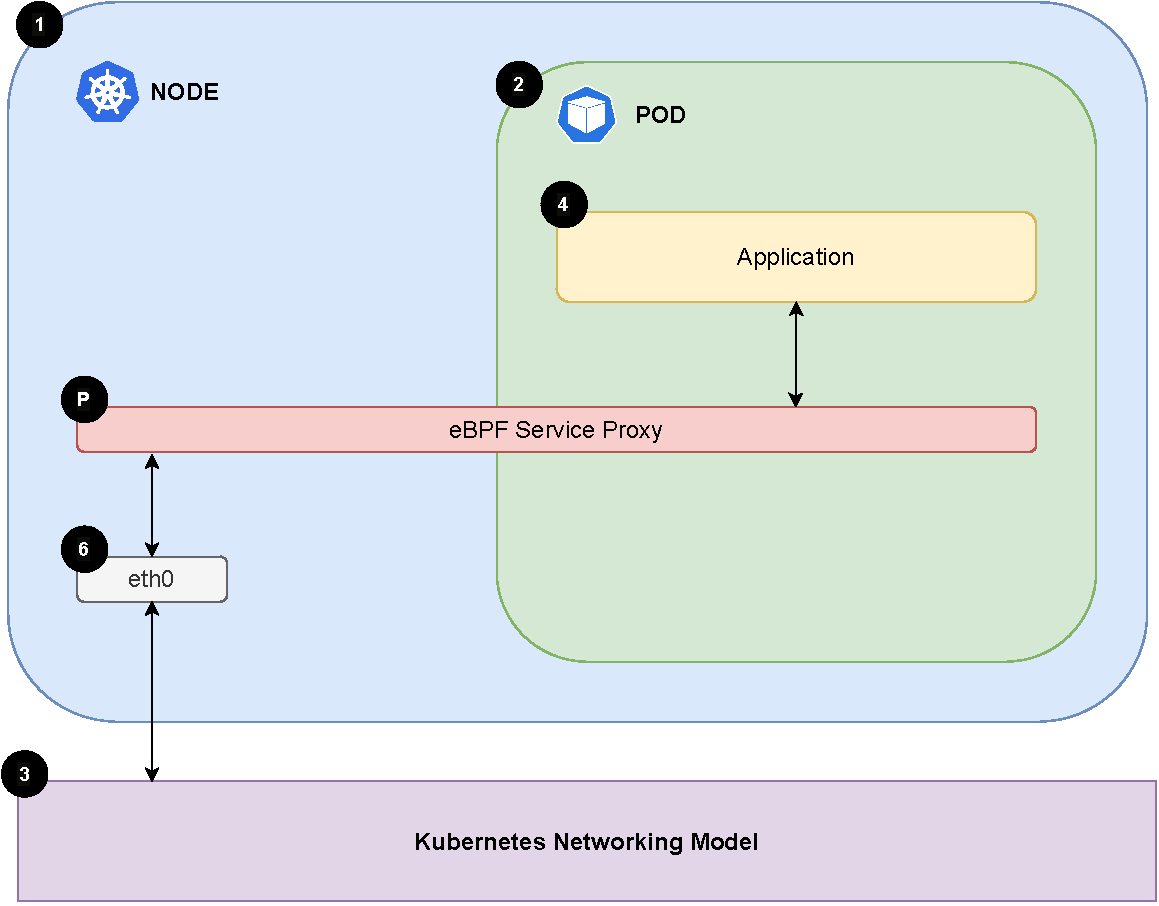
\includegraphics[width=\linewidth]{3_systems_survey/figures/sm-arch-ebpf.pdf}
    }
    
    \caption[\Gls{ebpf}-based data plane architecture.]{The data path of an \gls{ebpf}-based data plane.}
    \label{fig:sm-arch-ebpf}
\end{figure}


\subsection{Conclusion}
\label{sec:survey:analysis:conclusion}

To conclude the systems survey, we return to the initial research question (\ref{rq-1}), \textit{How do existing \gls{sm} implementations compare?}. The answer to this question is provided in various levels of detail throughout the systems survey. The most detailed and objective answer is provided  within the data synthesis and results section (\cref{sec:survey:results}) in which we identified domain-specific characteristics and features and compared the systems based on that. A summarized result is presented in the form of established functional and non-functional requirements (\cref{sec:survey:analysis}), in which we combine results from the data synthesis to provide a more generic, but more useful result. Finally, in \cref{sec:survey:analysis:architectures}, we take a deep-dive into the architectural differences of identified systems in which we answer the research question by exploring key characteristics in more detail.

Throughout this systems survey, we observed that \gls{sm} systems can have different approaches and goals and that systems within this the area are constantly changing. With many of the systems adopting different strategies and bleeding-edge technologies, the area is exciting in many ways. 